Nachdem die Wetterstation über MODBUS kommuniziert, soll in diesem Kapitel das MODBUS Protokoll näher erläutert werden. Dabei wird überwiegend Bezug auf die offizielle MODBUS Spezifikation genommen \cite{ModbusDoc}. Angesiedelt auf der ersten, zweiten und siebten Ebene des OSI Modells und damit einfach zu handhaben, ist MODBUS als Kommunikationsprotokoll in der Industrie weit verbreitet. Die unten stehende Abbildung \textbf{\ref{fig:prinzip}} dient zur ersten Orientierung der nachfolgend behandelten Themengebiete. 
\begin{figure}[hbtp]
\centering
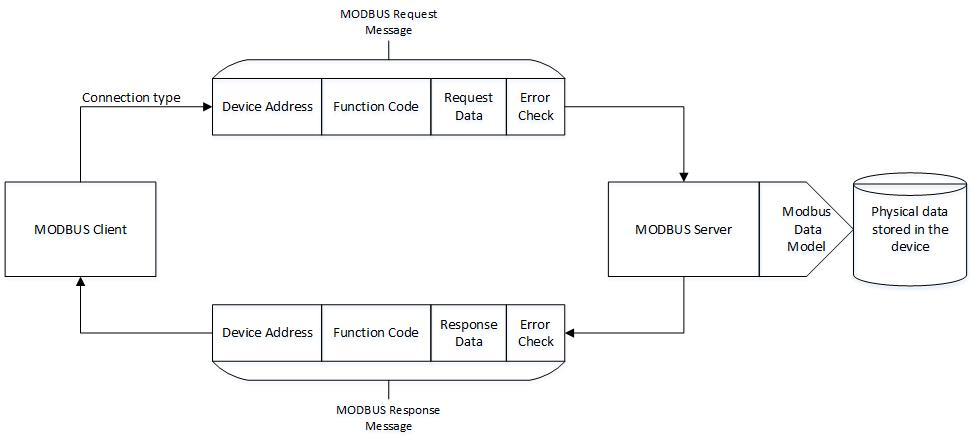
\includegraphics[scale=0.65]{modbus/msgskizze}
\caption{Skizze der Funktionsweise des MODBUS Protokolls}
\label{fig:prinzip}
\end{figure}
\section{Verbindungstypen}
Es ist möglich das Protokoll auf drei Verbindungstypen zwischen Client und Server einzusetzen. Dazu zählen: 
\begin{itemize}
\item eine Internetverbindung TCP/IP 
\item eine asynchrone serielle Verbindung (z.B. RS-232, RS-422, RS-485, etc.)
\item eine MODBUS Plus Verbindung  
\end{itemize}
In dieser Arbeit ist die Wetterstation seriell über eine RS-485 Schnittstelle mit dem Rechner verbunden. Die RS-485 Schnittstelle bietet den Vorteil, dass die Verbindung der Netzwerkteilnehmer wie bei einer RS-232 Schnittstelle nur über eine Zweidrahtleitung erfolgen kann. Jedoch können im Gegensatz zur RS-232 Schnittstelle bis zu 32 Teilnehmer im Netzwerk angeschlossen werden. Die Netzwerklänge kann ohne Verstärker bis zu 1200m betragen \cite{Schleicher.2008}. Diese Eigenschaften bieten sich an, um die Wetterstation wie in der Einleitung erwähnt, in ein Sensornetzwerk zu integrieren. Das Energiemanagementsystem kann die Daten entsprechend auslesen und Aktoren einstellen.
\section{Nachrichtenaufbau}
Wie eine typische MODBUS Nachricht aufgebaut ist, zeigt die unten stehende Abbildung \textbf{\ref{fig:modbusmessage}}. 
\begin{figure}[h]
\centering
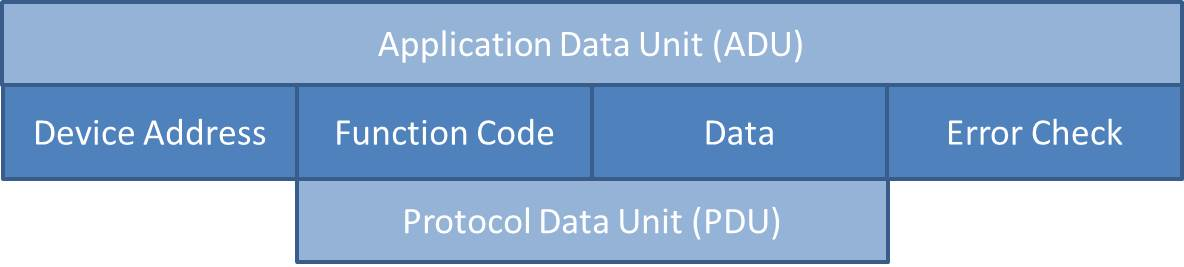
\includegraphics[scale=0.65]{modbus/ADUPDU}
\caption{Aufbau einer MODBUS Nachricht}
\label{fig:modbusmessage}
\end{figure} 
Die PDU ist unabhängig vom Netzwerk auf dem das Protokoll eingesetzt wird und setzt sich aus dem Funktionscode und den zu übermittelnden Daten zusammen. Mit einem Byte codiert gibt der Funktionscode an, ob eine schreibende oder lesende Kommunikation an welcher Art Register vorgenommen werden soll. Er kann aber auch einfach nur eine Aktion ausführen. In der Spezifikation werden drei Funktionscodearten genannt, öffentliche, benutzerdefinierte und reservierte Funktionscodes von denen in dieser Arbeit aber nur die Öffentlichen interessieren. Im Falle einer Anfrage des Client, enthält der Datenblock die entsprechenden Informationen über die genaue Adresse und Anzahl der zu lesenden oder beschreibenden Register. Für einen Schreibprozess wird hier auch der notwendige Input angegeben. Die abgefragten Daten des Servers sind ebenfalls im Datenblock untergebracht. Ein besonderes Augenmerk muss auf die Adressierung im Datenblock gelegt werden. Da hier nur die Startadresse angegeben wird und die Anzahl der nachfolgenden Adressen, ist es nicht möglich mit einer Nachricht nicht konsekutive Registeradressen auszulesen oder zu beschreiben. Hierfür wäre jeweils eine eigene Nachricht notwendig. Die Slave-ID und der Error-Check sind Informationen, die für das Netzwerk sprich den Verbindungstyp zwischen den Geräten eine Rolle spielen. Wie eben kurz skizziert, unterscheidet das MODBUS Protokoll zwischen drei Arten von PDUs, die nachfolgend zusammengefasst aufgeführt sind:
\begin{itemize}
\item die Anfrage-PDU besteht aus dem Funktionscode und den Anfragedaten
\item die Antwort-PDU besteht ebenfalls aus einem Funktionscode und den Antwortdaten
\item die Fehler-PDU besteht aus dem Fehlerfunktionscode (Funktionscode + 0x80 hex) und der Fehlermeldung 
\end{itemize}
Die Bytereihenfolge im Datenblock folgt der big-endian Anordnung, d.h. das Most Significant Bit kommt an erster und das Least Significant Bit an letzter Stelle. 
\section{Registertypen}
Die Daten, die vom Client abgefragt werden können, müssen physikalisch im Speicher des Servers liegen. Eine Verknüpfung dieses Speichers mit den zur Verfügung stehenden Registern im MODBUS Protokoll ermöglicht den Zugriff. Es werden vier Registerarten unterschieden, die in der Tabelle \textbf{\ref{tab:regartenmodbus}} aufgezeigt sind.
\begin{table}[htbp]
\caption{Übersicht der Registerarten im MODBUS Protokoll}
\rowcolors{1}{cyan}{white}
{
\setlength{\extrarowheight}{0.1cm}
\begin{tabular}{| l | l | l | p{6.5cm} |}
\hline
\textbf{Register} & \textbf{Wortlänge} & \textbf{Zugriff} & \textbf{Info}\\[0.5cm]
\hline \hline
\hiderowcolors
Diskreter Input & 1 Bit & Lesen & Daten werden durch ein I/O System bereitgestellt \\
Coils & 1 Bit & Lesen/Schreiben & Daten können über ein Anwendungsprogramm geändert werden \\
Input Register & 16 Bit & Lesen & Daten werden durch ein I/O System bereitgestellt \\
Holding Register & 16 Bit & Lesen/Schreiben & Daten können über ein Anwendungsprogramm geändert werden \\ 
\hline
\end{tabular}
}

\label{tab:regartenmodbus}
\end{table}
Jedes dieser Register besitzt einen Adressraum der bei 0 beginnt und bei 65535 endet. Zieht man noch eine weitere Quelle heran, so liegen die gültigen Adressbereiche jedoch anders verteilt vor. So besitzen die Coil-Register nur einen gültigen Adressraum von 1-9999, der Diskrete Input von 10001-19999, das Input Register von 30001-39999 und das Holding Register von 40001-49999 \cite{modicon}.    
\section{Nachrichtenverarbeitung}
Die Abbildung \textbf{\ref{fig:modbustransdiag}} im Anhang zeigt den Ablauf einer Nachrichtenüberprüfung und an welcher Position welcher Fehlercode gesendet wird, wenn die Nachricht fehlerhaft ist. 
\section{Funktions- und Fehlercodes}
Wie bereits erwähnt, ist der Funktionscode ein entscheidender Baustein in der MODBUS Nachricht. Es ist daher von Vorteil die für die Zwecke dieser Arbeit Wichtigen zu identifizieren, um das Handling des Programms zu vereinfachen. Die im Anhang dargestellte Abbildung \textbf{\ref{fig:fcodetab}} zeigt die zur Verfügung stehenden Funktionscodes. Gelb markiert sind dabei die Codes, die für die Kommunikation zwischen MATLAB und der Wetterstation Bedeutung haben. Bei Test hat sich zudem herausgestellt, dass die Services File Record Access, Diagnostics und Other für diese Hardware nicht gültig sind.    
Wie schon im Abschnitt~\ref{coilabfrage} auf Seite~\pageref{coilabfrage} beschrieben, müssen für den Fall einer Abfrage der Zustände des Temperatursensors oder der FSK Qualität die Coiladressen 0 oder 1 ausgelesen werden. Hierzu reicht es also jeweils eine Adresse in der MODBUS Nachricht anzugeben und die auszulesende Adresszahl auf 1 zu setzen. Die Anfrage- und Antwortnachricht für einen funktionierenden Temperatursensor ist in der Tabelle \textbf{\ref{tab:coilnachricht}} beispielhaft mit allgemeingültigen Ergänzungen dargestellt. Alle zwei Byte breiten Worte, wie zum Beispiel die Startadresse, setzen sich aus einem sogenannten High-Byte (H-Byte) und einem Low-Byte (L-Byte) zusammen.
\begin{table}[htbp]
\caption{Aufbau einer lesenden Kommunikation mit einem Coil-Register }
\rowcolors{1}{cyan}{white}
{
\setlength{\extrarowheight}{0.1cm}
\begin{tabular}{| l | l | l | p{7.5cm} |}
\hline
\textbf{\parbox[t]{2.6cm}{Nachrichten-\\typ}} & \textbf{\parbox[t]{2.6cm}{Nachrichten-\\teil}} & \textbf{\parbox[t]{1.7cm}{Wort-\\länge}} & \textbf{Inhalt}\\[0.25cm]
\hline \hline
\hiderowcolors
Anfrage & Funktionscode & 1 Byte  & 0x01 \\
 		& Startadresse  & 2 Bytes & H-Byte 0x00 L-Byte 0x00 (0x0000 bis 0xFFFF möglich) \\
        & Adressanzahl  & 2 Bytes & H-Byte 0x00 L-Byte 0x01 (1 bis 2000 (0x7D0) möglich) \\
Antwort & Funktionscode & 1 Byte  & 0x01 \\
		& Byteanzahl    & 1 Byte  & 0x01 (Ist das Ergebnis von Adressanzahl mod 8 = 0, so ergibt sich die Byteanzahl aus dem Ergebnis der Adressanzahl dividiert durch 8, andernfalls wird um ein Byte erhöht.)\\
		& Coil Status   & n Bytes & 0x01 (8 Coilzustände werden mit einem Byte, hier 00000001 angezeigt. Das Most Significant Bit im Antwort Byte steht dabei für die höchste Registeradresse.)\\ 
\hline
\end{tabular}
}
\label{tab:coilnachricht}
\end{table} 
\begin{table}[htbp]
\caption{Aufbau einer schreibenden Kommunikation mit einem Holding-Register }
\rowcolors{1}{cyan}{white}
{
\setlength{\extrarowheight}{0.1cm}
\begin{tabular}{| l | l | l | p{7.5cm} |}
\hline
\textbf{\parbox[t]{2.6cm}{Nachrichten-\\typ}} & \textbf{\parbox[t]{2.6cm}{Nachrichten-\\teil}} & \textbf{\parbox[t]{1.7cm}{Wort-\\länge}} & \textbf{Inhalt}\\[0.25cm]
\hline \hline
\hiderowcolors
Anfrage & Funktionscode    & 1 Byte  & 0x06\\
 		& Registeradresse  & 2 Bytes & H-Byte 0x00 L-Byte 0x70 (0x0000 bis 0xFFFF möglich)\\
        & Registerinput    & 2 Bytes & H-Byte 0x01 L-Byte 0x61 (0x0000 bis 0xFFFF möglich)\\
Antwort & Funktionscode    & 1 Byte  & 0x06\\
		& Registeradresse  & 2 Byte  & H-Byte 0x00 L-Byte 0x70\\
		& Registerinput    & 2 Byte  & H-Byte 0x01 L-Byte 0x61\\ 
\hline
\end{tabular}
}
\label{tab:writehreg}
\end{table}
\begin{table}[htbp]
\caption{Aufbau einer lesenden Kommunikation mit einem Holding-Register }
\rowcolors{1}{cyan}{white}
{
\setlength{\extrarowheight}{0.1cm}
\begin{tabular}{| l | l | l | p{7.2cm} |}
\hline
\textbf{\parbox[t]{2.6cm}{Nachrichten-\\typ}} & \textbf{\parbox[t]{2.6cm}{Nachrichten-\\teil}} & \textbf{\parbox[t]{1.7cm}{Wort-\\länge}} & \textbf{Inhalt}\\[0.25cm]
\hline \hline
\hiderowcolors
Anfrage & Funktionscode  & 1 Byte      & 0x03\\
 		& Startadresse   & 2 Bytes     & H-Byte 0x00 L-Byte 0x00 (0x0000 bis 0xFFFF möglich)\\
        & Adressanzahl   & 2 Bytes     & H-Byte 0x00 L-Byte 0x5F (1 bis 125 (0x7D) möglich)\\
Antwort & Funktionscode  & 1 Byte      & 0x03\\
		& Byteanzahl     & 2 Byte      & 2 x N (N = Adressanzahl)\\
		& Registeroutput & N x 2 Bytes & \\ 
\hline
\end{tabular}
}
\label{tab:readhreg}
\end{table}
Ein weiterer wichtiger Funktionscode ist der Code 0x06, mit dem man in das Holding-Register Werte schreiben kann. Wie im Abschnitt~\ref{comsetreg} auf Seite~\pageref{comsetreg} in der Tabelle \ref{tab:kommeinstpara} nachzulesen, wird die zu beobachtende Wetterregion mit einem Wert im Holdingregister an der Adresse 112 festgelegt. Für die Definition der Wetterregion München (Wert 353) ist die hierzu notwendige Kommunikation in der Tabelle \ref{tab:writehreg} als Beispiel skizziert. Der wohl wichtigste und am meisten verwendete Funktionscode in dieser Arbeit ist der Code 0x03 zum Lesen des Holding-Registers. Über ihn werden sämtliche Prognosedaten ausgelesen. Auch hier soll ein Beispiel in der Tabelle \ref{tab:readhreg} den Aufbau verdeutlichen. In dem gezeigten Beispiel werden alle Wetterdaten, insgesamt 96 Werte, für die Mittlere Temperaturprognose abgerufen. Schlägt ein Kommunikationsprozess fehl, so wird vom Server statt der Antwortnachricht eine Fehlernachricht gesendet. Es sind folgende Fehlernachrichten vorgesehen:
\begin{itemize}
\item Code 01 Ungültige Funktion
\item Code 02 Ungültige Adressdaten
\item Code 03 Ungültige Daten
\item Code 04 Fehler beim MODBUS Server
\end{itemize}
Code 1 kann auftreten, wenn die entsprechende Funktion im Gerät nicht implementiert ist oder der Server sich in einem falschen Zustand befindet. Code 02 wird dann gesendet, wenn in der Anfrage mehr Register ausgelesen werden sollen, als zur Verfügung stehen. Code 03 gibt an, dass es sich bei dem im Datenblock befindlichen Wert um einen für den Server nicht Gültigen handelt. Code 04 wird übermittelt, wenn beim Server während der Bearbeitung der Anfrage ein Fehler aufgetreten ist.    
\section{Cyclic Redundancy Check}
Im MODBUS Protokoll sind zwei Modi definiert, wie die Nachrichten aufgebaut sein können. Da die Wetterstation aber im RTU Modus betrieben wird, braucht man sich in dieser Arbeit über den ASCII Modus keine Gedanken machen. Die Methode zum Absichern der Datenintegrität im RTU Modus ist der Cyclic Redundancy Check. Der Master sendet die MODBUS Nachricht an den Client, der wiederum den CRC Wert aus der Slave-ID, und der ADU berechnet. Kommt er auf ein anderes Ergebnis als es im CRC Wert steht, wird er die Anfrage nicht beantworten und es kommt zu einem Fehler, den der Master lösen muss.\cite{modicon} 

Analog dem Algorithmus aus dem Buch \enquote{Digitale Schnittstellen und Bussysteme} wird in MATLAB die CRC Prüfsumme berechnet. Zunächst wird die Nachricht aus Slave-ID und PDU (\textit{modbus\_pud\_hex}) an die Funktion \textsf{crc\_calc} übergeben. Die Länge dieser Nachricht geteilt durch zwei ergibt die Anzahl Bytes. Diese müssen im nächsten Schritt auf ein entsprechend breites binäres Bit Wort transformiert werden. Danach erfolgt die Initialisierung des Ausgangsschieberegisters, des Generatorpolynoms und der beiden Bytepositionszeiger \textit{m} und \textit{n}. Die MODBUS Nachricht wird durch die erste for-Schleife byteweise bearbeitet. Dabei werden die einzelnen Bytes zuerst auf 16 Bit breite Worte gebracht indem Nullen der rechten Seite zugewiesen werden. Danach folgt eine Exklusiv-Oder-Verknüpfung mit dem Ausgangsschieberegister 0xFFFF hex. Jetzt erfolgt für jedes Bit im aktuell anstehenden Byte ein Rechtsschieben bis das erste Bit mit einer eins herausgeschoben wurde. Die frei werdenden Bits auf der linken Seite werden mit Nullen aufgefüllt. Im nächsten Schritt wird mit dem Generatorpolynom wieder eine Exklusiv-Oder Operation durchgeführt und die Prozedur wird mit dem Ergebnis fortgesetzt. Am Ende wird das Resultat \textit{crc\_erg} dem Schieberegister zugewiesen und die Bytepositionszeiger erhöht. Sind alle Schleifen durchlaufen, wird zum Schluss das Schieberegister in einen 2 Byte hex Wert transformiert und mit der Slave-ID und der PDU zur ADU (\textit{txdata\_hex}) verknüpft.\cite{Schleicher.2008} 
\lstinputlisting[firstline=1, lastline=51]{modbus/crccalc.m}
\section{Simulation der Wetterstation}  
Nachdem nun die MODBUS und Wetterstationsspezifikation analysiert wurden, kann man mit der Umsetzung des MATLAB Programmes beginnen. Für den Fall, dass man noch nie in MATLAB mit einer seriellen Schnittstelle gearbeitet hat, bietet es sich an, diese zunächst einmal zu simulieren. Hierzu wurden in dieser Arbeit zwei Programme verwendet. Das eine Programm simuliert den COM Port des MODBUS Slave, heißt \enquote{Virtual Serial Ports Emulator} und wird von \enquote{eterlogic.com} zum Download angeboten \cite{eterlogic}. Das andere Programm virtualisiert den MODBUS Slave selbst und heißt \enquote{PeakHMI MODBUS Serial RTU slave}. Anbieter hierfür ist die Firma Everest Software LLC \cite{everest}. Der große Vorteil in der Simulation liegt darin, dass man in das virtualisierte Holdingregister an eine bestimmte Adresse Werte schreiben kann. Mit den Methoden von MATLAB kann man nun versuchen diesen Wert auszulesen. Mit dieser Methodik kann man schnell die Funktionalität des erarbeiteten Codes auch offline erproben. 

     
      
